%% %%%%%%%%%%%%%%%%%%%%%%%%%%%%%%%%%%%%%%%%%%%%%%%%%%%%%%%%%%%%%%%%%%%%%%%%%%%
%%
%%          $Id: general_rules.tex 420 2013-04-08 15:30:35Z holz $
%%    author(s): RoboCupAtHome Technical Committee(s)
%%  description: description of the GENERAL RULES
%%
%% %%%%%%%%%%%%%%%%%%%%%%%%%%%%%%%%%%%%%%%%%%%%%%%%%%%%%%%%%%%%%%%%%%%%%%%%%%%
\chapter{General Rules \& Regulations}
\label{chap:rules}

These are the general rules and regulations for the competition in the RoboCup@Home league.
Every rule in this section can be considered to implicitly include the 
term \emph{``unless stated otherwise''}, meaning that additional or contrary rules in particular
test specifications have a higher priority than those mentioned herein in the general rules and regulations.  

%%%%%%%%%%%%%%%%%%%%%%%%%%%%%%%%%%%%%%%%%%%%%%%%%%%%%%%%%
\section{Team Registration and Qualification}


\subsection{Registration and Qualification Process}
\label{rule:participation}

Each year there are four phases in the process toward participation:
\begin{enumerate}
	\item \iterm{Intention of Participation} (optional)
	\item \iterm{Preregistration} 
	\item \iterm{Qualification} announcements
	\item Final \iterm{Registration} for qualified teams
\end{enumerate}
Positions 1 and 2 will be announced by a call on the \iterm{RoboCup@Home mailing list}. Preregistration requires a \iterm{team description paper}, a \Term{video}{qualification video} and a \Term{website}{Team Website}.

\subsection{Qualification Video}
As a proof of running hardware, each team has to provide a \iterm{qualification video} showing at least all from following abilities (minimum requirement):
\begin{itemize}
	\item Human-Robot interaction
	\item Navigation (safe, indoors with obstacle avoidance).
	\item Object detection \& manipulation.
	\item People detection
	\item Speech recognition.
	\item speech synthesis (clear and loud).
\end{itemize}

Showing some of the following abilities is recommended:
\begin{itemize}
	\item Activity recognition
	\item Complex speech recognition
	\item Complex action planning
	\item Gesture recognition
\end{itemize}

For qualification, we consider showing the robot(s) successfully solving at least one test of the last year's or current rulebook (excluding ability tests).

For robots moving slowly, it is much appreciated speed-up videos. When doing so, please specify the speed factor being used (e.g.~2x, 5X, 10X). The same is applied for slow motion scenes.

We encourage teams to produce self-explicative videos for a general audience where complex tasks are solved

Please notice that the videos should not last longer than the average time for a test (max.~\SI{30}{\minute}).

\subsection{Team Website}

The \iterm{Team Website} should be designed for a broader audience, but also including scientific material and access to open source code being developed. Requirements are as follows:

\begin{enumerate}

	\item \textbf{Multimedia: } Please include as many photos and videos of the robot(s) as possible.

	\item \textbf{Language: } The team website has to be in English. Other languages may be also available, but English must be default language.

	\item \textbf{Team: } List of the team members including brief profiles.

	\item \textbf{RoboCup:} Link to the league website and previous participation of the team in RoboCup.

	\item \textbf{Scientific approach: } The team website has to include research lines, description of the approaches, and information on scientific achievements.

	\item \textbf{Publications: } Relevant \iterm{publications} from 5 years up to date. Downloadable publications are scored higher during the qualification process.

	\item \textbf{Open source material: } Blueprints, designs, repositories or any kind of contribution to the league is highly scored during qualification process.
\end{enumerate}


\subsection{Team Description Paper}
\label{rule:website_tdp}

The \iaterm{team description paper}{TDP} must have a explained description of your main research, including the scientific contribution, goals, scope, and results.

Preferably, it should also contain the following:
\begin{itemize}
	\item the focus of research and the contributions in the respective fields, 
	\item innovative technology (if any), 
	\item re-usability of the system for other research groups
	\item applicability of the robot in the real world
	\item photo(s) of the robot(s)
\end{itemize}

~\\\noindent On the last page, after references, please include:
\begin{itemize}
	\item Name of the team
	\item contact information
	\item website
	\item team members
	\item photo(s) of the robot(s), unless included before.
	\item description of the hardware used 
	\begin{itemize}
		\item Provide a brief compact list (2DOF head, 2x7DOF anthropomorphic arms, Pioneer base, etc.).
		\item Avoid explaining how your hardware works unless it is part of your research (e.g.~we already know what a Hokuyo Laser or Kinect are used for).
	\end{itemize}
	\item description of the software
	\begin{itemize}
		\item Provide a brief compact list (ROS, ROS nav2d, Object Recognition Kitchen, OpenCV, etc.).
		\item Avoid explaining how your software works unless it is part of your research.
		\item List the \iterm{external computing resources} (See \refsec{rule:robot_external_computing}), if any. State their purpose and URL/IP-address. 
	\end{itemize}
\end{itemize}

~\\\noindent The TDP has to be in English, up to eight pages in length and formatted according to the guidelines of the RoboCup International Symposium. It goes into detail about the technical and scientific approach.

Please notice that, during qualification process, TDP will be scored by its scientific value, novelty and contributions.


%% %%%%%%%%%%%%%%%%%%%%%%%%%%%%%%%%%%%%%%%
\subsection{Qualification}
\label{rule:qualification}

During the \iterm{qualification process} a selection will be made by the \iaterm{Organizing Committee}{OC} Taken into account and evaluated in this decision process are:
\begin{itemize}
	\item The content on the team website, scoring higher publications and open content;
	\item the number of abilities shown in the qualification video,
	\item the complexity of the tasks shown in the qualification video, and
	\item the scientific value, novelty and contributions in the \iterm{team description paper}. %, and
	% \item the information in the \iterm{RoboCup\char64Home Wiki} (added by the team).
\end{itemize}
(Additional) evaluation criteria are: 
\begin{itemize}
	\item the performance in previous competitions, 
	\item the relevant scientific contributions and publications, and
	\item the contributions to the RoboCup@Home league.
\end{itemize}

% For getting considered in the evaluation, be sure to insert your team's name when adding information to the \iterm{RoboCup\char64Home Wiki}.    


% Local Variables:
% TeX-master: "../Rulebook"
% End:


%%%%%%%%%%%%%%%%%%%%%%%%%%%%%%%%%%%%%%%%%%%%%%%%%%%%%%%%%
\section{Scenario}
\label{sec:scenario}

The tests take place in the \iterm{RoboCup@Home arena}. In addition, particular tests are situated outside the arena, e.g., in a previously unknown public place. The following rules are related to the \iterm{RoboCup@Home arena} and its contents. 

\subsection{RoboCup@Home arena}
The \iterm{RoboCup@Home arena} is a realistic home setting consisting of inter-connected rooms like, for instance, a living room, a kitchen, a bath room, and a bed room. 

% \subsection{Team area}\label{rule:scenario_team_area}

% \todo{remove? does not depend on the rules, but on local organization }
% The maximum number of people to register per team is unlimited, but
% the organization only provides space for \emph{four} (4) persons to
% work at tables in the team area. 
% \todo{this is actually more an additional note for the registration information}

\subsection{Walls, doors and floor}
\label{rule:scenario_walls}

The indoor home setting will be surrounded by high and low \Term{walls}{Arena walls}. These walls will be built up using standard fair construction material.

\begin{enumerate}
	\item \textbf{Walls:} Walls have a minimum height of \SI{60}{\centi\meter}. A maximum height is not specified, but should be chosen so that the audience is able to watch the competition.\\
	Walls will be fixed and are likely to be not modified during the competition (see \refsec{rule:scenario_changes}). 

	\item \textbf{Doors:} There will be at least two entry/exit \Term{doors}{Arena doors} connecting the outside of the scenario. These doors are used as starting points for the robots (see \refsec{rule:start_position}).
	% At least one of the entrances will be a door with a handle (not a knob).\
	There will be also another door inside the scenario with a handle (not a knob) between any two rooms. Doors with handle (not a knob) may be closed at any time, it is expected robots be able to open them.

	\item \textbf{Floor:} The floor of the arena as well as the doorways of the arena are even. That is, there will be no significant steps or even stairways. However, minor unevenness such as carpets, transitions in floor covering between different areas, and minor gaps (especially at doorways) must be expected.

	\item \textbf{Appearance:} Floor and walls are mainly uni-colored but can contain texture, e.g., a carpet on the floor, or a poster or picture on the wall.\\
	Although being unlikely at the moment, transparent elements are also possible. 
\end{enumerate}


\subsection{Furniture}
\label{rule:scenario_furniture}

The arena will be equipped with typical objects (furniture) that are not specified in quantity and kind. The minimal configuration consists of 
\begin{itemize}
	\item a small dinner table with two chairs, 
	\item a couch, 
	\item an open cupboard or small table with a television and remote control, 
	\item a cupboard or shelf (with some books inside), and
	\item a refrigerator in the kitchen (with some cans and plastic bottles inside). 
\end{itemize}
A typical arena setup is shown in \reffig{fig:scenario_arena}.

\begin{figure}[tbp]
	\centering
	\subfloat[Typical arena]{\label{fig:scenario_arena}
\includegraphics[height=46mm]{images/typical_arena.jpg}} ~ 
	\subfloat[Typical objects]{\label{fig:scenario_objects}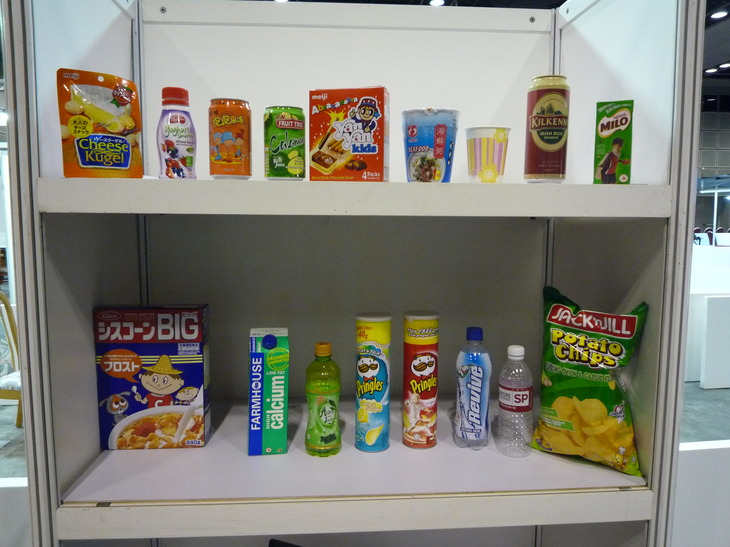
\includegraphics[height=46mm]{images/typical_objects.jpg}}
	\caption{Scenario examples: (a) a typical arena, and (b) typical objects.}
	\label{fig:arena}
\end{figure}



\subsection{Changes to the arena}
\label{rule:scenario_changes}

Since the robots should be able to function in the real world the scenario is not fixed and might change without further notice.
\begin{enumerate}
	\item \textbf{Major changes:} 
	The arena is meant to be a simulated apartment. 
	The furniture might be moved around between challenges. 
	This includes furniture that is a named location (see \refsec{rule:scenario_names}).
	As in a normal home, furniture is not very likely to move from one room to another and is unlikely to be moved to the other side of a room.
	However, a couch or table may be rotated, moved to its side etc. 
	Walls will stay in place and rooms will not change function.
	Passages might be blocked and cleared. 
	One hour before a test slot begins no \iterm{major changes} will be made.

	\item \textbf{Minor changes:} In contrast to major changes, \iterm{minor changes} like, for instance, slightly moved chairs cannot be avoided and may happen at any time (even during a test). 
\end{enumerate}


%%%%%%%%%%%%%%%%%%%%%%%%%%%%%%%%%%%%%%%%%%%%%%%%%%%%%%%%%%%%%%%%%%
%
% Objects section.
%
% Revisited by Mauricio Matamoros for 2015
%
%%%%%%%%%%%%%%%%%%%%%%%%%%%%%%%%%%%%%%%%%%%%%%%%%%%%%%%%%%%%%%%%%%
\def\NumObjects{10\ }
\def\NumLocations{20\ }
\def\NumNames{20\ }

\subsection{Objects}
\label{rule:scenario_objects}
Some tests in the RoboCup@Home league involve object manipulation and recognition. These \iterm{objects} resemble items usually found in household environments like, for instance, soda cans, coffee mugs or books. An example of objects used in a previous competition can be seen in \reffig{fig:scenario_objects}.

Objects are divided in five main groups:

\begin{enumerate}
	\item \textbf{\iterm{Known objects}:} Objects with no noticeable difference among peers. \textit{Known objects} tend to be artificial and regular shaped, such as coke cans, beer bottles, cereal boxes, etc.~A set of copies of these objects is provided before the competition for training.

	\item \textbf{\iterm{Alike objects}:} Objects with slight differences among peers (e.g.~color, size, shape). \textit{Alike objects} tend to be natural and similar to each other, but not equal; for example: apples, bananas, rags, etc.~A specimen of these objects is provided before the competition for training.

	\item \textbf{\iterm{Containers}:} Objects which can contain, transport or be filled with other objects or their content, such as trays, baskets, bowls, etc.~. As with \textit{known objects}, \textit{containers} are known beforehand with no noticeable difference among peers, and a copy is provided before the competition for training.

	\item \textbf{\iterm{Special objects}:} Objects require a proper identification and special handling (not necesarily grasping), operation or interaction for accomplishing a particular task. Examples of special objects are: door handles, chairs, walking sticks, poles, etc.~Notice that a copy of these objects may not be available beforehand for previous training.

	\item \textbf{\iterm{Unknown objects}:} Any other object that is not known beforehand but can be grasped or handled.
\end{enumerate}

The following general rules for objects apply:

\begin{enumerate}
	\item \textbf{Object category:} Each object will be assigned to an \iterm{object category}. The objects \quotes{apple} and \quotes{banana} may be of class \quotes{fruits} for example.

	\item \textbf{Object (category) locations:} An \iterm{object location} object will be assigned to each\iterm{object category}. For example, Objects categorized as \quotes{fruits} may be usually found on the \quotes{kitchen table}, and unknown objects \quotes{unknown} may be usually found on the \quotes{trash bin}.

	\item \textbf{Announcement:} The TC makes the set of \iterm{objects}, including their names, categories, and usual locations; available during the setup days. 
	
	\item \textbf{Placement:} \nterm{object placement} Unless stated otherwise, in manipulation tasks, the objects will be positioned at \iterm{manipulation locations} and less than \SI{15}{\centi\meter} away from the border of the surface they are located at. There will be at least \SI{5}{\centi\meter} space around each object.
\end{enumerate}

\paragraph*{Important note:} It is not allowed to modify any of the objects provided for training. Also, teams are not allowed to keep more than 5 the objects provided for training at a time nor retaining it for more than one hour.

\subsubsection{Containers}
The TC will provide at least two containers (a transport container such as a tray and a pouring container such as a bowl) which will be available for training during the setup days.

There are no restrictions on a container size, appearance or weight; however, it can be expected that the selected containers be lightweight, with handles, and easily manipulable by a human using both hands.

\paragraph*{Custom containers.}
\label{rule:custom_containers}
The goal of containers is to encourage \textbf{bi-hand manipulation}. However, it is allowed that a team provide a \iterm{custom container} adapted to be used by the robot, considering the following:
\begin{enumerate}
	\item Custom containers must be approved by the TC during during the \iterm{Robot Inspection} (see \refsec{sec:robot_inspection}).
	\item Custom containers must \emph{not} have any kind of artificial marks, sensors, or electronic devices.
	\item Penalties may apply for the use of custom containers. The TC may establish special penalties during the \iterm{Robot Inspection}. The default penalties applicable to any task involving a container are as follows.
	\begin{itemize}
	\item Special color on an otherwise unmodified two-hand manipulable container: 75\% of the points.
	\item Special color on an otherwise unmodified single-hand manipulable container: 50\% of the points.
	\item Specially designed or adapted two-hand manipulable container (e.g.~special handles): 50\% of the points.
	\item Specially designed or adapted single-hand manipulable container (e.g.~special handle): 25\% of the points.
	\item Two-hand manipulable container adapted to be used \textit{single-handed}: 25\% of the points.
	\item On-robot mounted container: 0 points.
	\end{itemize}
	\textbf{Notes:} Trays are considered two-hand manipulable containers, while most bowls and dishes are considered single-hand manipulable container unless they are too big. Color patterns are allowed as long as they look natural (e.g.~\textit{barber sign colored} handles are allowed, but black and white bar-code like handles are not). Penalties does not stack, the most meaningful modification is considered. 
\end{enumerate}

\subsubsection{Predefined objects}
The TC will compile a list of at least \NumObjects objects (including both \iterm{known objects} and \iterm{alike objects}) which will be available for training. There are no restrictions on an object size, appearance or weight; however, it can be expected that the selected objects are easily manipulable by a human using a single hand.

Note that, any object not previously announced by the TC is automatically considered an unknown object for scoring purposes (e.g.~ornamentation).

%%%%%%%%%%%%%%%%%%%%%%%%%%%%%%%%%%%%%%%%%%%%%%%%%%%%%%%%%%%%%%%%%%
%
% Predefined locations section.
%
%%%%%%%%%%%%%%%%%%%%%%%%%%%%%%%%%%%%%%%%%%%%%%%%%%%%%%%%%%%%%%%%%%

\subsection{Predefined locations}
\label{rule:scenario_locations}

Some tests in the RoboCup@Home league involve \iterm{predefined locations}. 
These may include places like a \quotes{bookshelf} or a \quotes{dining table}, as well as certain objects such as a \quotes{television}, or the \quotes{front door}. 

\begin{enumerate}
	\item \textbf{Definition:} The TC will compile a list of predefined locations. There are no restrictions on which parts of the arena will be selected as a predefined location.

	\item \textbf{Location classes:} Each location will be assigned to a \iterm{location class}. The objects \quotes{couch} and \quotes{arm chair} may be of class \quotes{seat} for example. 

	\item \textbf{Announcement:} The TC makes the set of locations (and their names and classes) available during the setup days.

	\item \textbf{Position:} The positions of locations are \emph{not} necessarily fixed (see \refsec{rule:scenario_changes}).

	\item \textbf{Manipulation locations:} The TC will mark at least \NumLocations locations out of the set of predefined locations as being \iterm{manipulation locations}. Whenever a test involves manipulation, the object to manipulate will be placed at one of the manipulation locations. 
\end{enumerate}



\subsection{Predefined rooms}
\label{rule:scenario_rooms}
Some tests in the RoboCup@Home league involve \iterm{predefined rooms}. 
\begin{enumerate}
	\item \textbf{Definition:} The TC will compile a list of room names.
	\item \textbf{Announcement:} The TC makes the set of rooms available during the setup days.
\end{enumerate}



\subsection{Predefined (person) names}\label{rule:scenario_names}

Some tests in the RoboCup@Home league involve \iterm{predefined names} of people. 

\begin{enumerate}
	\item \textbf{Definition:} The TC will compile a list of \NumNames predefined names. The names are \SI{50}{\percent} male and \SI{50}{\percent} female, and taken from the (current) most common first names in the United States.\\
	In order to ease speech recognition, it is tried to select names to be phonetically different from each other.

	\item \textbf{Announcement:} The TC makes the set of names available during the setup days.
	\item \textbf{Assignment:} When a test involves interacting with persons (using a person's name), all involved persons are assigned names by the referees before the test. 
\end{enumerate}

Typical names are, for example, James, John, Robert, Michael and William as male names; Mary, Patricia, Linda, Barbara and Elizabeth as female names.


%% %%%%%%%%%%%%%%%%%%%%%%%%
\subsection{Wireless network}
\label{rule:scenario_wifi}

For wireless communication, an \iterm{arena network} is provided. The actual infrastructure depends on the local organization. 

\begin{itemize}
	\item To avoid interference with other leagues, this WiFi has to be used for communication only. It is not allowed to use the above or any other WiFi network for personal use at the venue.
	\item During the competitions, only the active team is allowed to use the \iterm{arena network}. 
	\item The organizers cannot guarantee reliability and performance of wireless communication. Therefore, teams are required to be ready to setup, start their robots and run the tests even if, for any reason, network is not working properly.
\end{itemize}

Preferably the organizers will try to provide one LAN cable on the desk of each participating team for Internet connection. However, this cannot be guaranteed. If multiple LAN connections are needed, each team has to bring its own LAN hub/switch and cables.

\paragraph*{Important note:} Any unapproved wireless device may be removed by the TC at any time.

\subsection{Smart Home Devices}
\label{rule:smarthomedevices}

The Organizing and Technical Committees in coordination with the Local Organization will compile a list of \iterm{Smart~Home} official devices that will be available in the arena and can be used in some tests for additional score.

At any time, only the Smart~Home devices provided by the Local Organization and approved by the Technical Committee may be used during competition.

\subsubsection{Smart~Home devices list announcement}
The list if Smart~Home devices will be provided to teams as soon as it becomes available and has been granted by the Local Organization and approved by the Technical Committee. 

This list must be announced at least one month prior the competition. In case that this list does not become available for that date, Smart~Home devices may still be present at the arena for testing, but no additional score can be achieved for its use. This is to maintain fair conditions among all teams.

\subsubsection{Technical specifications}
The list of \iterm{Smart~Home} official devices will include as much technical information as possible. However, before it becomes available you may assume the following considerations:

\begin{enumerate}
	\item \textbf{Interface:} Most Smart~Home devices interface wireless, often via R/F transmitters. When possible, the OC will provide an official interface via the \iterm{arena network}.
	\item \textbf{Operating voltage:} The operating voltage used will be the standard for the place of the competition (e.g.120V/60Hz for North America and 220V/50Hz for Europe). Please note that devices designed for other voltages/frecuencies may burn when plugged to the outlet.
	\item \textbf{Type of devices:} Mostly Smart~Home switches will be used (set on/off, read can not be guaranteed). For high bandwidth devices such as microphones or video cameras, an official interface (such as a ROS topic or web service) will be provided via the \iterm{arena network}.
\end{enumerate}

\subsubsection{Availability \& Scoring}
All test has been designed to optionally allow the use of Smart~Home devices and even grant bonus scoring for using this option. However, robots must be able to continue operating normally when there are no Smart~Home devices available. Therefore, it is unacceptable that a robot stuck while trying to operate those devices.

As stated in \refsec{rule:scenario_wifi}, organizers cannot guarantee reliability and performance of wireless communication. Therefore, in case of malfunction or communication problems with the Smart~Home devices, or any other issue which may affect scoring, no claims will be accepted by the EC/TC/OC, nor test will be repeated. The decision on if a team given points for using \iterm{Smart~Home} devices, is conducted by the \iaterm{Technical Committee}{TC}, and it reserves the rights of discarding Smart~Home related scoring.


% Local Variables:
% TeX-master: "../Rulebook"
% End:


%%%%%%%%%%%%%%%%%%%%%%%%%%%%%%%%%%%%%%%%%%%%%%%%%%%%%%%%%
\section{Robots}
\label{rule:robots}

\subsection{Autonomy \& Mobility}
Robots that participate in the RoboCup@Home league need to be \Term{autonomous}{Autonomy} and \Term{mobile}{Mobility}. Any deviations reported to the TC, may result in a penalty for the team (see \refsec{rule:extraordinary_penalties}).


\subsection{Number of robots}
\label{rule:robots_number}

\begin{enumerate}
	{\bf\item Registration:} The maximum \term{number of robots} per team that can be registered for the competitions is \emph{two} (2).
	{\bf\item Regular Tests:} Only one robot is allowed per test. For different tests different robots can be used.
	{\bf\item Open Demonstrations:} In the \iterm{Open Challenge} and the \iterm{Finals} both robots can be used simultaneously.
	{\bf\item RoboZoo:} In the \iterm{RoboZoo} both robots can be used simultaneously as long as they fit into the cage.
\end{enumerate}


\subsection{Size and weight of robots}
\label{rule:robots_size}

\begin{enumerate}
	{\bf\item Dimensions:} The dimensions of a robot should not exceed the limits of an average door, which is \SI{200}{\centi\meter} by \SI{70}{\centi\meter} in most countries.\\ 
	The TC may allow the qualification and registration of larger robots, but due to the international character of the competition it cannot be guaranteed that the robots can actually enter the arena. In case of doubt, contact the local organization. 
	{\bf\item Weight:} There is no specific weight restriction. However, the weight of the robot and the pressure it exerts on the floor should not exceed local regulations for the construction of buildings which are used for living and/or offices in the country where the competitions is being held.
	{\bf\item Transportation:} Team members are responsible for quickly moving the robot out of the arena.	If the robot cannot move by itself (for any reason), the team members must be able to transport the robot away with an easy and fast procedure.
\end{enumerate}



\subsection{Emergency stop button}
\label{rule:robots_emergency_button}

\begin{enumerate}
	{\bf\item Accessibility and visibility:} Every robot has to provide an easily accessible and visible \iterm{emergency stop} button. 
	{\bf\item Color:} It must be coloured red, and preferably be the only red button on the robot. If it is not the only red button, the TC may ask the team to tape over or remove the other red button. 
	{\bf\item Robot behavior:} When pressing this button, the robot and all parts of it have to stop moving immediately.
	{\bf\item Inspection:} The emergency stop button is tested during the \iterm{Robot Inspection} test (see \refsec{sec:robot_inspection}).
\end{enumerate}



\subsection{Start button}
\label{rule:start_button}

\begin{enumerate}
	{\bf\item Requirements:} As stated in \refsec{rule:start_signal}, teams that aren't able to carry out the default start signal (opening the door) have to provide a \iterm{start button} that can be used to start tests. The team needs to announce this to the TC before every test that involves a start signal, including \iterm{Robot Inspection}.
	{\bf\item Definition:} The start button can be any \quotes{one-button procedure} that can be easily executed by a referee.  This includes, for example, the release of the \iterm{emergency button} (\refsec{rule:robots_emergency_button}), a hardware button different from the \iterm{emergency button} (e.g., a green button), or a software button in a Graphical User Interface. 
	{\bf\item Inspection:} It is during the the \iterm{Robot Inspection} test (see \refsec{sec:robot_inspection}) that the procedure for the start button, if needed, is announced to the TC and inspected. The start button for a robot should be the same for all the tests.
	{\bf\item Penalty for using start button:} If a team needs to use the start button in a test where opening the door is the start signal, it may receive a penalty (see \refsec{rule:start_signal}).
\end{enumerate}



\subsection{Appearance and safety}
\label{rule:roobt_appearance}

Robots should have a nice product-like appearance, be safe to operate and should not annoy its human users. The following rules apply to all robots and are part of the \iterm{Robot Inspection} test (see \refsec{sec:robot_inspection}). 
\begin{enumerate}
	{\bf\item Cover:} The robot's internal hardware (electronics and cables) should be covered in an appealing way. The use of (visible) duct tape is strictly prohibited.
	{\bf\item Loose cables:} There may not be any loose cables hanging out of the robot. 
	{\bf\item Safety:} The robot may not have sharp edges or other things that could severe people.
	{\bf\item Annoyance:} The robot should not permanently make loud noises or use blinding lights.
\end{enumerate}




\subsection{Audio output plug}\label{rule:roobt_audio_out}

\begin{enumerate}
	{\bf\item Mandatory plug:} Either the robot or some external device connected to it \emph{must} have a \iterm{speaker output plug}. It is used to connect the robot to the sound system so that the audience and the referees can hear and follow the robot's speech output.
	{\bf\item Inspection:} The output plug needs to be presented to the TC during the \iterm{Robot Inspection} test (see \refsec{sec:robot_inspection}).
	{\bf\item Audio during tests:} Audio (and speech) output of the robot during a test have to be understood at least by the referees and the operators.
	\begin{compactitem}
		\item It is the responsibility of the teams to plug in the transmitter before a test, to check the sound system, and to hand over the transmitter to next team.
		\item Do not rely on the sound system! For fail-safe operation and interacting with operators make sure that the sound system is not needed, e.g., by having additional speakers directly on the robot.
\end{compactitem}
\end{enumerate}


% Local Variables:
% TeX-master: "../Rulebook"
% End:


\section{Data Recording}
  \label{rule:datarecording}
  In order to benchmark robots and software outside the RoboCup@Home arena, the teams are asked to contribute to a public dataset.
  This will consist of audio, imagery and other data obtained and generated by the robots during RoboCup@Home challenges.
  Contributing to this dataset gives a small bonus as an incentive. 
  The bonus will be proportional to the points gathered normally: 
    if 50\% of points are gathered, 50\% of the data collection points are awarded. 
    
  \subsection{Collected data}
    During a challenge, specific data is to be gathered and stored on a USB stick. 
    After all attempts at a challenge are made, the USB stick must be given to the TC, which will copy the data to the public dataset.
    The recordings themselves are not used for scoring and may be post-processed manually to be more useful, before handing over to the TC. 
    Not all types of data are interesting for each challenge and thus each challenge will list which data to record. 
    
    \begin{itemize}
    \item \textbf{Audio: } A .wav file of conversation or commands given by any operator and the result of the automatic speech recognition, if applicable.
      The recording must be made of the same signals that are input to the automatic speech recognition software. 
      \begin{itemize}
	\item \textbf{Format: } TeamName\_SensorName\_Timestamp.wav
	\item \textbf{Format: } PCM Wav 44.1 kHz 16 bit stereo
      \end{itemize}
      
    \item \textbf{Commands: } A text file with the commands as received by the robot. 
      This may be the output of speech recognition or the outcome of any form of the continue rule.
      Include a timestamp and then the command. 
      \begin{itemize}
	\item \textbf{Format: } TeamName\_commands\_Timestamp.csv
	\item \textbf{Format: } csv-file. First column has command timestamp, second column the command in ``quotes''.
      \end{itemize}
    
    \item \textbf{Images: } 2D and/or 3D RGB(D) images from the robot's camera(s) while doing any sort of recognition task.
			    Record the full field of view. 
    \begin{itemize}
      \item
	\textbf{Color images: } 
	\begin{itemize}
	  \item \textbf{Filename: } TeamName\_SensorName\_Timestamp\_rgb.png
	  \item \textbf{Format: } Standard PNG 24bit
	\end{itemize}
      \item
	\textbf{Depth images: } 
	\begin{itemize}
	  \item \textbf{Filename: } TeamName\_SensorName\_Timestamp\_depth.png
	  \item \textbf{Format: } Standard PNG 16bit grayscale
	\end{itemize}
    \end{itemize}
    
    \item \textbf{Mapping data: } Record the data the robot uses for mapping its surroundings and obstacle avoidance plus the resulting map. 
      For many robots this will be 2D laser scans of an Laser Range Finder but other means are possible. 
    
    \item \textbf{Plans: } Any plan generated by the robot. This includes navigation paths, arm trajectories and action plans. 
      If possible, plans are preferably annoted with whether is was succesfully executed or not.
    \end{itemize}
    
    For ROS-based robots, the most convenient data format for mapping data (laser scans, occupancy grids etc.) and motion plans are their ROS messages recorded into a ROS Bag file.
    This ROSBag should then contain:
     \begin{itemize}
       \item \textbf{Laser scans: } sensor\_msgs/LaserScan
       \item \textbf{Path(s): } nav\_msgs/Path
       \item \textbf{Map(s): } nav\_msgs/OccupancyGrid
       \item \textbf{Robot pose: } geometry\_msgs/PoseStamped
       \item \textbf{Transformation tree: } tf2\_msgs/TFMessage or equivalent
       \item \textbf{Odometry: } nav\_msgs/Odometry
      \end{itemize}
    Although not all robots use ROS, this serves as a guideline of the type of data that may be interesting for others. 
    The RoCKIn robot competition provides a conversion tool that converts to ROS Bag files:
    \url{http://rockinrobotchallenge.eu/rockin_d2.1.3.pdf}, section 3.4 and 
    \url{https://github.com/rockin-robot-challenge/benchmark_and_scoring_converter}

%   
%   5
% In the following, ‘offline’ identifies data produced by the robot that will be collected by the referees when
% the execution of the benchmark ends (e.g., as files on a USB stick), while ‘online’ identifies data that the robot
% has to transmit to the testbed during the execution of the benchmark. Data marked neither with ‘offline’ nor
% with ‘online’ is generated outside the robot. NOTE: the online data should also be displayed by the robot on its
% computer screen, for redundancy purposes, in case problems with wireless communications arise.
% 
% 6Speech files from all teams and all benchmarks (both Task benchmarks and Functional benchmarks) will be
% collected and used to build a public dataset. The audio files in the dataset will therefore include all the defects of
% real-world audio capture using robot hardware (e.g., electrical and mechanical noise, limited bandwidth, harmonic
% distortion). Such files will be usable to test speech recognition software, or (possibly) to act as input during the
% execution of speech recognition benchmarks.
% 
% Catering to Granny_annie's comfort:
% • On the robot, the audio signals of the conversations between Annie and the robot. [offline]
% • The final command produced during the natural language analysis process. [online]
% • The pose of the robot while moving in the environment.
% • The pose of the robot while moving in the environment, as perceived by the robot. [offline]
% • The sensorial data of the robot when recognizing the object to be operated. [offline]
% • The results of the robot’s attempts to execute Annie’s commands.
% 
% Welcoming Visitors:
% The event/command causing the activation of the robot. [online]
% • The video signal from the door camera.
% • The pose of the robot during the execution of the task.
% • The pose of the robot while moving in the environment, as perceived by the robot. [offline]
% • The results of any attempts by the robot to detect and classify a visitor. [online]
% • The audio signals of the conversations with the visitors. [offline]
% • Any notifications from the robot (e.g., alarm if a visitor shows anomalous behavior). [online]
% • The results of any actions taken by the robot, including opening or closing the front door,
% guiding visitors into and around the apartment, manipulating objects, etc.
% 
% Getting to know my home:
% The output files produced by the robot, as described by section 4.3.4. [offline]
% • The pose of the robot during the execution of the task.
% • The pose of the robot while moving in the environment, as perceived by the robot. [offline]
% • The result (success/failure) of the command issued to the robot.

%%%%%%%%%%%%%%%%%%%%%%%%%%%%%%%%%%%%%%%%%%%%%%%%%%%%%%%%%
\section{External devices}\label{rule:roobt_external_devices}
\begin{enumerate}
	{\bf\item Definition:} Everything which is not part of the robot is considered an \iterm{external device}. 
	{\bf\item Inspection:} In general, external devices are not allowed unless presented and explained to the \iaterm{Technical Committee}{TC} during the \iterm{Robot Inspection} test (see \refsec{sec:robot_inspection}).
	{\bf\item Supervision:} In regular tests, external devices may only be used under supervision by referees and after approval by the TC. The devices have to be brought to the arena for every test, and removed quickly after the test.
	{\bf\item Open demonstrations:} For the \iterm{Open Challenge}, \iterm{RoboZoo}, and the \iterm{Finals}, external devices are allowed, still their use needs to be announced beforehand.
	{\bf\item Wireless devices:} All \iterm{wireless devices} including bluetooth devices, walkie-talkies, and anything else that uses an RF signal to operate need to be announced to the \iaterm{Organizing Committee}{OC}. The use of any wireless device not approved by the TC is strictly prohibited.  
	{\bf\item Artificial landmarks:} \iterm{Artificial landmarks} and \iterm{markers} are not allowed.
	{\bf\item Computing devices:} External computers for decentralized computations are allowed, but have to be inside the arena, i.e.,~not on its periphery.
	{\bf\item Wireless LAN:} The use of networks other than the \iterm{arena network} (see \refsec{rule:scenario_wifi}) is strictly prohibited.
	{\bf\item External microphones: }\iterm{External microphones}, hand microphones, and headsets are not allowed. Using an \iterm{on-board microphone} is mandatory for communication with the robot.
\end{enumerate}


%%%%%%%%%%%%%%%%%%%%%%%%%%%%%%%%%%%%%%%%%%%%%%%%%%%%%%%%%
\section{External computing}\label{rule:robot_external_computing}
Robots are allowed to use some form of external computing, for example in the form of so-called ``Cloud services'' and/or ``Internet API's'' etc. 
\begin{enumerate}
	\item \textbf{Definition:} Computing resources that are not physical part of the robot are \iterm{external computing resources}. 
	\item \textbf{Inspection:} In general, external computers are not allowed unless explained to and allowed by the \iaterm{Technical Committee}{TC}.
	  A team must announce to the TC at least 1 month in advance the external computing resources they want to use, for what purpose and how to reach the resources.
	  E.g. specify the URL or IP-address. 
	  This must be specified in the team description paper. 
	\item \textbf{Connection:} The robot may connect to \iterm{external computing resources} via a network connection, e.g. the Internet. 
	  The competition organisation cannot make any guarantees concerning availability, connectivity and performance of the connection. 
	  The robot should still be functional (albeit limited perhaps) if the \iterm{external computing resources} cannot be used for some reason.
	  This is the team's responsibility. 
	\item \textbf{Autonomy:} The robot has to maintain full autonomy when using \iterm{external computing resources}, 
	  meaning there may not be a human giving the robot any kind of instructions via \iterm{external computing resources}.
	  It is up to the team to prove to the \iaterm{Technical Committee}{TC} that there was no cheating introduced via the \iterm{external computing resources}. 
	  For example, the use of Amazon Mechanical Turk to classify and recognize objects during a competition will be considered cheating, since effectively a human will do the classification.
	  Remote control or tele-operation is also considered cheating. 
	\item \textbf{Availability:} The resources must be publicly available, for use by robots of other teams, well before and after the competition.
	\item \textbf{Recognition:} In case the resources are not developed by the team itself, the creators must be properly credited in the Team Description Paper (See \refsec{rule:website_tdp}).
	\item \textbf{Limit:} A robot is limited to use up to 5 \iterm{external computing resources}. 
\end{enumerate}


% Local Variables:
% TeX-master: "../Rulebook"
% End:
 


%%%%%%%%%%%%%%%%%%%%%%%%%%%%%%%%%%%%%%%%%%%%%%%%%%%%%%%%%
\section{Organization of the competition}
\label{sec:procedure_during_competition}

\subsection{Stage system}\label{rule:stages}

The competition features a \iterm{stage system}. It is organized in two stages each consisting of a number of specific tests. It ends with the \iterm{Finals}.

\begin{enumerate}
	\item \textbf{Stage~I:} The first days of the competition will be called \iterm{Stage~I}. 
	All qualified teams can participate in \iterm{Stage~I}. Stage~I comprehends a set of \iterm{Ability Tests}, an \iterm{Integration Test}, and an audience demonstration called \iterm{Following \& Guiding}. 
	Those \iterm{Proficency Tests} (\iterm{Ability Tests}, and \iterm{Integration Test}) are performed multiple times (See \refsec{rule:score_system}). 

% MAURICIO @2017: With the inclusion of SPL only 6 teams per league advance to the second stage (leagues are intended to have 13 teams).
	\item \textbf{Stage~II:} The best \emph{50\% of teams with full integrated capabilities}\footnote{If the total number of teams is less than 12, up to 6 teams may advance to Stage~II} (after Stage~I) advance to \iterm{Stage~II}. Here, more complex abilities or combinations of abilities are tested. In order to advance to Stage~II a team must successfully solve 3 out of \iterm{Proficency Tests} in Stage~I. \\
	The \iterm{Open Challenge} is the open demonstration in Stage~II.
% MAURICIO @2017: With the inclusion of SPL, we want the finals with no more than 6 teams. At this point, the best two of each league advance to the finals.
	\item \textbf{Final demonstration:} The best \emph{two teams} of each league, the ones with the highest score after Stage~II, advance to the final round. The final round features only a single open demonstration.
\end{enumerate}

% MAURICIO: No technical challenge since 2015
% In addition, a Technical Challenge (see \refsec{sec:TechnicalChallenge}) is carried out between Stage~II and the Final Demonstration, and its schedule is outside the scope of the Stage system.
In case of having no considerable score deviation between a team advancing to the next stage and a team dropping out, the TC may announce additional teams advancing to the next stage.


% MAURICIO @2017: With the inclusion of SPL, we make mandatory participating in at least one Stage II test to advance to the finals
\subsection{Number of tests}\label{rule:number_of_tests}
None of the tests is mandatory, except for the \iterm{Robot Inspection} test (see \refsec{sec:robot_inspection}). However, in order to participate in the finals, a team must have participated in at least one test of the Stage~II.


%%%%%%%%%%%%%%%%%%%%%%%%%%%%%%%%%%%%%%%%%%%%%%%%%%%%%%%%%
\subsection{Schedule}
\label{rule:schedule}

\begin{enumerate}
	\item \textbf{Tests:} The \iaterm{Organizing Committee}{OC} provides schedules for all tests and teams. 
	\item \textbf{Participation is default:} Teams have to indicate to the \iaterm{Organizing Committee}{OC} in which tests they are \emph{not} going to participate. Without such indication, they are automatically added to all test schedules and may receive a penalty when not attending (see \refsec{rule:not_attending}).
	\item \textbf{Slots:} The tests will be held in \iterm{test slots} of approximately two hours.
	\item \textbf{Preparation:} The \iaterm{Organizing Committee}{OC} provides schedules for all teams to organize the access to the arena between test slots. In these \iterm{preparation slots} the teams may conduct calibration procedures, remap the arena if necessary, or conduct test runs.
	Preparation slots are inserted whenever possible, but may not be available before all test slots. 
	\item \textbf{Arena access:} One hour before a test slot, only the teams participating in that slot are allowed in the arena.
This rule only applies when not having organized \iterm{preparation slots}.   
\end{enumerate}


%%%%%%%%%%%%%%%%%%%%%%%%%%%%%%%%%%%%%%%%%%%%%%%%%%%%%%%%%
%\subsection{Score system}\label{rule:score_system}
%
%\begin{enumerate}
%  \item \textbf{Stage~I:} The maximum total score per test in Stage~I is \scoring{2000 points}.
%  \item \textbf{Stage~II:} The maximum total score per test in Stage~II is \scoring{2600 points}.
%  \item \textbf{Special tests:} Tests may specify a maximum total score deviating from the general maximum total scores.  
%  \item \textbf{Minimum score:} The minimum total score per test in Stage~I and Stage~II is \scoring{0 points}. 
%  That is, if the total score for a test is below zero, the team does not receive any points.
%  \item \textbf{Penalties:} An exception to the \emph{minimum score} rule are penalties. 
%  Both penalties for not attending (see \refsec{rule:not_attending}) and extraordinary 
%  penalties (see \refsec{rule:extraordinary_penalties}) can cause a total negative score. 
%  \item \textbf{Partial scores:} All tests---except for the open demonstrations---are rewarded on a partial scoring basis. 
%  \begin{enumerate}
%  \item Tests are split into designated parts.
%  \item Each part is assigned a certain number of points.
%  \item A team that successfully passes a designated part of the test receives points for that part.
%  \item In case of partial success, referees (and TC members) may decide to only award a percentage instead of the full partial score.  
%  \item The total score for a test is the sum of partial scores.
%  \item Partial scores can be negative (e.g.~to penalize failures etc.).
%  \end{enumerate}
%\end{enumerate}

% MAURICIO: Explained Score System
\subsection{Score system}
\label{rule:score_system}

\begin{enumerate}
	\item \textbf{Stage~I:} The maximum total score (excluding special penalties and bonuses) in \iterm{Stage~I} is \scoring{1150 points}.
	% \item \textbf{Stage~I:} The maximum total score (excluding special penalties and bonuses) in \iterm{Stage~I} is \scoring{1050 points}.
	\begin{enumerate}
		\item \textbf{\iterm{Proficency Tests}:} Each proficiency test is attempted three times. The maximum total score is calculated as the average of the best two attempts for that test.
		% \item \textbf{Poster Session:} The Poster Session score is counted in Stage~I and may grant up to \scoring{50 points}.
	\end{enumerate}

	\item \textbf{Stage~II:} Test in \iterm{Stage~II} are rewarded on a task-solved scoring basis.
	\begin{enumerate}
		\item Each test but the \iterm{Open Challenge} has a main task. The base score for solving the main task is \scoring{250 points}.
		\item The maximum score for \iterm{Open Challenge} is \scoring{250 points}.
		\item Optionals and subtasks add bonus points to the main task score.
	\end{enumerate}

	\item \textbf{\iterm{Finals}:} Final score is normalized and special evaluation is used

	\item \textbf{Special tests:} Tests may specify a maximum total score deviating from the general maximum total scores.

	\item \textbf{Minimum score:} The minimum total score per test in \iterm{Stage~I} and \iterm{Stage~II} is \scoring{0 points}. That is, if the total score for a test is below zero, the team does not receive any points.

	\item \textbf{Penalties:} An exception to the \emph{minimum score} rule are penalties. Both penalties for not attending (see \refsec{rule:not_attending}) and extraordinary penalties (see \refsec{rule:extraordinary_penalties}) can cause a total negative score. 

	\item \textbf{Partial scores:} All tests---except for the open demonstrations---are rewarded on a partial scoring basis. 
	\begin{enumerate}
		\item Tests are split into designated parts.
		\item Each part is assigned a certain number of points.
		\item A team that successfully passes a designated part of the test receives points for that part.
		\item In case of partial success, referees (and TC members) may decide to only award a percentage instead of the full partial score.  
		\item The total score for a test is the sum of partial scores.
		\item Partial scores can be negative (e.g.~to penalize failures etc.).
	\end{enumerate}
\end{enumerate}


%%%%%%%%%%%%%%%%%%%%%%%%%%%%%%%%%%%%%%%%%%%%%%%%%%%%%%%%%
% MAURICIO: On 2015, Open Challenge moved to Stage 2. There is no Demo Challenge
\subsection{Open Demonstrations}
\label{sec:open-demonstrations}
\begin{enumerate}
	\item \textbf{Stage~II:} The \iterm{Open Challenge} is the open demonstration in \iterm{Stage~II}.
	\begin{enumerate}
		\item To participate in the \iterm{Open Challenge}, a team needs to participate in at least one regular \iterm{Stage~II} test.
		\item Teams can demonstrate freely chosen abilities. 
		\item The performance is evaluated by a jury consisting of the \iaterm{Technical Committee}{TC}.
		\item The \iterm{Open Challenge} is described in \refsec{sec:test_open_challenge}.
	\end{enumerate}

	% \item \textbf{Stage~II:} The \iterm{Demo Challenge} is the open demonstration in Stage~II.
	% \begin{enumerate}
	% \item To participate in the Demo Challenge, a team needs to participate in at least one regular Stage~II test.
	% 	\item The scope (and topic) of the Demo Challenge are defined by the TC on a yearly basis.
	% 	\item Teams can demonstrate freely chosen abilities, but according to the scope. 
	% 	\item The performance is evaluated by the \iaterm{Technical Committee}{TC}.
	% 	\item The Demo Challenge is described in \refsec{sec:test_demo_challenge}.
	% \end{enumerate}
	
	\item \textbf{\iterm{Finals}:} The competition ends with a final demonstration.
	\begin{enumerate}
		\item The concept of the final demonstration is the same as that of the \iterm{Open Challenge}, but the performance evaluation is different. 
		\item The are two juries---an \emph{external} consisting of three or more people not from the RoboCup @Home league, and an \emph{internal} formed by the \iaterm{Executive Committee}{EC}. Both juries have different sets of evaluation criteria.
		\item Members of the external jury are selected by the \iaterm{Executive Committee}{EC} on site. 
		\item The demonstration in the \iterm{Finals} does not have to be different from the one shown in the \iterm{Open Challenge}. It does not have to be the same either.
	\end{enumerate}
\end{enumerate}


% Local Variables:
% TeX-master: "../Rulebook"
% End:


%%%%%%%%%%%%%%%%%%%%%%%%%%%%%%%%%%%%%%%%%%%%%%%%%%%%%%%%%
\section{Procedure during Tests}

\subsection{Safety First!}
\label{rule:safetyfirst}
\begin{enumerate}
	\item \textbf{Emergency Stop:} At any time when operating the robot inside and outside the scenario the owners have to stop the robot immediately if there is a remote possibility of dangerous behavior towards people and/or objects. 
	\item \textbf{Stopping on request:} If a referee, member of the Technical or Organizational committee, an Executive or Trustee of the federation tells the team to stop the robot, there will be no discussion and the robot has to be stopped \emph{immediately}.
	\item \textbf{Penalties:} If the team does not comply, the team and its members will be excluded from the ongoing competition immediately by a decision of the RoboCup@Home \iaterm{Technical Committee}{TC}. 	Furthermore, the team and its members may be banned from future competitions for a period not less than a year by a decision of the RoboCup Federation Trustee Board.
\end{enumerate}

\subsection{Maximum number of team members}
\label{rule:number_of_people}
\begin{enumerate}
	\item \textbf{Regular Tests:} During a regular test, the maximum number of team members allowed inside the arena is \emph{one} (1). The only exceptions are tests that require for more team members in the arena.
	\item \textbf{Setup:} During the setup of a test, the number of team members inside the arena is not limited.
	% \item \textbf{Open Demonstrations:} During the \iterm{Open Challenge} \iterm{Demo Challenge}, and the \iaterm{final demonstration}{Finals}, the number of team members inside the arena is not limited.
	\item \textbf{Open Demonstrations:} During the \iterm{Open Challenge}, and the \iaterm{final demonstration}{Finals}, the number of team members inside the arena is not limited. 
	\item \textbf{Moderation:} During a regular test, one team member \emph{must} be available to host and comment the event (see \refsec{rule:moderator}).
\end{enumerate}

\subsection{Fair play}
\label{rule:fairplay}
\iterm{Fair Play} and cooperative behavior is expected from all teams during the entire competition, in particular:
\begin{itemize}
	\item while evaluating other teams, 
	\item while refereeing, and 
	\item when having to interact with other teams' robots.  
\end{itemize}
This also includes:
\begin{itemize}
	\item not trying to cheat (e.g.~pretending autonomous behavior where there is none), 
	\item not trying to exploit the rules (e.g.~not trying to solve the task but trying to score), and 
	\item not trying to make other robots fail on purpose. 
\end{itemize}
Disregard of this rule can lead to penalties in the form of negative scores, and disqualification for a test or even for the entire competition. 

\subsection{Robot Autonomy and Remote Control}
\begin{enumerate}
	\item \textbf{No touching:} During a test, the participants are not allowed to make contact with the robot(s), unless it is in a \quotes{natural} way and/or required by the test specification. 
	\item \textbf{Natural interaction:} The only allowed means to interact with the robot(s) are gestures and speech.
	\item \textbf{Natural commands:} Only general instructions are allowed. 
	Anything that resembles direct control is prohibited.
	\item \textbf{Remote Control:} Remotely controlling the robot(s) is strictly prohibited. This also includes pressing buttons, or influencing sensors on purpose.
	\item \textbf{Penalties:} Disregard of these rules can lead to penalties in the form of negative scores, and disqualification for a test or even for the entire competition. 
\end{enumerate}

\subsection{Collisions}
\begin{enumerate}
	\item \textbf{\iterm{Touching}:} Robots are allowed to gently \emph{touch} objects, items and humans. 	They are not allowed to crash into something. The \quotes{safety first} rule (\refsec{rule:safetyfirst}) supercedes all other rules.
	\begin{itemize}
		\item It \emph{is} allowed however to \emph{functionally} touch an item with e.g.~the base.
	\end{itemize}
	The OC/TC/EC and the RoboCup Trustees all have the right to immediately stop a robot, and to disqualify a team for the duration of the competition, or longer, in case of \emph{dangerous} behavior. Furthermore, referees can recommend to disqualify a team in which case EC/TC decides.
	\item \textbf{\iterm{Major collisions}:} If a robot crushes into something during a test, the robot is immediately stopped.	Additional penalties may apply. 
	\item \textbf{Robot-Robot avoidance:} If two robots encounter each other, they both have to actively try to avoid the other robot.
	\begin{enumerate}
		\item A robot which is not going for a different route within a reasonable amount of time (e.g., \SI{30}{\second}) is removed.
		\item A non-moving robot blocking the path of another robot for longer than a reasonable amount of time (e.g., \SI{30}{\second}) is removed. In this context, \quotes{moving} refers to any kind of motion or action required in the test. For example, a robot standing still but manipulating an object does not need to stop manipulating and move away, even when blocking the way of another robot for the duration of the manipulation.
	\end{enumerate}
\end{enumerate}



\subsection{Removal of robots}
\label{rule:robot_removal}
Robots not obeying the rules are stopped and removed from the arena.
\begin{enumerate}
	\item It is the decision of the referees and the TC member monitoring the test if and when to remove a robot.
	\item When told to do so by the referees or the TC member monitoring the test, the team has to immediately stop the robot, and remove it from the arena without disturbing the ongoing test.
\end{enumerate}


\subsection{Start signal}
\label{rule:start_signal}

\begin{enumerate}
	\item \textbf{Opening the door:} Unless stated otherwise, the cue for the robot to enter the arena and start the test is the opening of the door by a referee.
	\item \textbf{Start button:} If the robot is not able to automatically start after opening the door, the team may start the robot using a start button. 
	\begin{enumerate}
		\item Using a start button needs to be announced to the referees. It is the responsibility of the team to do so before the test starts.
		\item There may be penalties for using a start button in some tests
	\end{enumerate}
\end{enumerate}


\subsection{Entering and leaving the arena}
\label{rule:start_position}
\begin{enumerate}
	\item \textbf{Start position:} Unless stated otherwise, the robot starts outside of the arena.
	\item \textbf{Entering:} The robot has to autonomously enter the arena.
	\item \textbf{Success:} The robot is said to \emph{have entered} when the door used to enter can be closed again, and the robot is not blocking the passage.
\end{enumerate}



\subsection{Gestures}
\label{rule:gestures}
Hand gestures may be used to control the robot in the following way:
\begin{enumerate}
	\item \textbf{Definition:} The teams define the hand gestures by themselves. 
	\item \textbf{Approval:} Gestures need to be approved by the referees and TC member monitoring the test. Gestures should not involve more than the movement of both arms. This includes e.g.~expressions of sign language or pointing gestures.
	\item \textbf{Instructing operators:} It is the responsibility of the team to instruct operators.
	\begin{enumerate}
		\item The team may only instruct the operator when told to so by a referee.
		\item The team may only instruct the operator in the presence of a referee.
		\item The team may only instruct the robot for as long as allowed by the referee.
		\item When the robot has to instruct the operator, it is the robot that instructs the operator and \emph{not} the team. The team is not allowed to additionally guide the operator, e.g., tell the operator to come closer, speak louder, or to repeat a command.
		\item The robot is allows to instruct the operator at any time.
	\end{enumerate}
	\item \textbf{Receiving gestures:} Unless stated otherwise, it is not allowed to use a speech command to set the robot into a special mode for receiving gestures.
\end{enumerate}



\subsection{Referees}
\label{rule:referees}
% \refmark{}
\begin{enumerate}
	\item \textbf{Setup:} Unless stated otherwise, each test is monitored by two referees and one member of the \iaterm{Technical Committee}{TC}.
	\item \textbf{Selection:} The two referees 
	\begin{itemize}
		\item are chosen by EC/TC/OC, 
		\item are announced together with the schedule for the test slot, 
		\item and have to referee all teams in that slot.
		\item Referees may not be from one of the teams in the slot.
	\end{itemize}
	\item \textbf{Not showing up:} Not showing up for refereeing (on time) will result in a penalty (see \refsec{rule:extraordinary_penalties}). 
	\item \textbf{TC monitoring:} The referee from the TC acts as a main referee. 
	\item \textbf{Referee instructions:} Right before each test, referee instructions are conducted by the TC. The referees for all slots need to be present at the arena where the referee instructions are taking place.When and where referee instructions are taking place is announced together with the schedule for the slots.
\end{enumerate}


\subsection{Operator}
\label{rule:operator}
\begin{enumerate}
	\item \textbf{Default operator:} Unless stated otherwise, robots are operated by the monitoring TC member, a referee, or by a person selected by the TC.
	\item \textbf{Fallback/custom operator:} If the robot fails to understand the command given by the default operator, the team may continue with a custom operator.
	\begin{compactitem}
		\item The custom operator may be any person chosen by the team (and willing to do so); including the referees or the monitoring TC member. 
		\item A penalty may be involved when using a custom operator.
	\end{compactitem}
\end{enumerate}



\subsection{Moderator}
\label{rule:moderator}
\begin{enumerate}
	\item \textbf{Providing a moderator:} For each regular test (i.e., not for the open demonstrations), all participating teams need to provide a team member as moderator for the duration of their performance. 
	\item \textbf{Responsibilities:} The moderators have to:
	\begin{compactitem}
		\item explain the rules of the test, 
		\item comment on the performance of their team, 
		\item not interfere with the performance, 
		\item speak in English, 
		\item and obey the instructions by the monitoring TC member.
	\end{compactitem}
	\item \textbf{Competitive tests:} In competitive tests (tests in which two teams directly compete against each other), the moderation has to be done by the two teams together.
\end{enumerate}


\subsection{Time limits}
\label{rule:time_limits}
\begin{enumerate}
	\item \textbf{Stage~I:} Unless stated otherwise, the time limit for each test in \iterm{Stage~I} is \timing{5 minutes}.
	\item \textbf{Stage~II:} Unless stated otherwise, the time limit for each test in \iterm{Stage~II} is \timing{10 minutes}.
	\item \textbf{Setup time:} Unless stated otherwise, all time specifications, e.g., setup time and time for instructing operators, are within the total test time. 
	\item \textbf{Scores:} When the time is up, the team has to immediately remove their robot(s) from the arena; no more points can be scored. In special cases, the monitoring TC member may ask the team to continue the test for demonstration purposes (after time is up, points cannot be scored). 
\end{enumerate}



\subsection{Restart}
\label{rule:restart}
\begin{enumerate}
	\item \textbf{Stage 1} has no restarts but features multiple attempts at a challenge. 
	If a robot fails during an attempt, the attempt ends. 
	A robot has several (ideally 3, depending on available time in the scheduele) attempts for each challenge. An attempt cannot be restarted. 
	E.g. if a robot fails halfway through an attempt at the navigation challenge, the attempt is over, the robot is moved out of the test area and may prepare for the remaining attempts at the challenge.

	\item \textbf{Stage 2} does have restarts for challenges:
	\begin{enumerate}
		\item \textbf{Number of restarts:} A team may request one (1) restart during a test, unless stated in otherwise. There are tests in which a restart is not allowed.
		\item \textbf{Procedure:} In case a restart is allowed, the team may request the restart only before 50\% of the time alloted to the test. The complete test is then restarted from the beginning (e.g., with entering the arena). The referees may rearrange the locations of objects/persons if necessary.
		\item \textbf{Time:} The time is neither restarted nor stopped. The team has 1 minute to restart the test (the same time to start the test); if the team is not able to do so in the allotted time, the test is called as finished by the TC.
		\item \textbf{Score:} The score of the second run (after the restart) counts. If it is lower than the score of the first run (before the restart), the average score of first and second run is taken.
		\item \textbf{Forced restart:} The referees and the monitoring TC member may force the team to do a restart:
		\begin{compactitem}
			\item if the robot is doing nothing or nothing reasonable for \timing{one minute}, or
			\item when the robot fails to understand a command for \timing{five times}, or
			\item after a minor collision
		\end{compactitem}  
	\end{enumerate}
\end{enumerate}


\subsection{Continue rule: Bypassing Automatic Speech Recognition}
\label{rule:asrcontinue}

Giving commands to the robot is an important part of many tests. 
RoboCup@Home fosters natural human-robot interaction through gestures and speech, such that speech is the primary modality to give complex commands to the robot. 
Automatic speech recognition (ASR) however can be very difficult in the international competition environment of RoboCup. 
Because active robots are preferred over robots that are passive due to failing ASR, 
  the team is allowed to provide means to bypass ASR. 
The robot can then still continue to a next part of a test, but with a penalty for needing a bypass. 
The penalty for using such a bypass will be more severe in future competitions.

All robots are \textbf{highly recommended to use QR-codes as a standardized alternative} to ASR. These QR-codes will be generated by the TC to encode the spoken command/sentence as-is. 
Any punctuation like commas, questionmarks, apostrophes and dots in the (generated) spoken command will also be present in the QR-code. 

Non-standardized alternative means should be
  % declared in the registration form and
  approved by and demonstrated to the TC during the \iterm{Robot Inspection} test (see \refsec{sec:robot_inspection}).

\subsubsection{Procedure}
Automatic Speech Recognition is preferred and any command given to the robot will given by voice first.
\begin{enumerate}
\item \textbf{Default:} When the referee generates a command for the robot, it will be read out loud by the operator to the robot. 100\% of the points gained in the execution of the command will be awarded.
\item \textbf{team member: } If this fails, a team member may speak the command to the robot if this was not the case already.  75\% of the points gained in the execution of the command will be awarded, if not stated otherwise.
\item \textbf{QR-code:} If this fails as well, as a last resort, a QR-code will be generated that encodes the command as plain text and shown to the robot, displayed on either a piece of paper or a computer screen. 90\% of the total points will be awarded if a QR-code was necessary. 
\end{enumerate}

\begin{enumerate}
	\item \textbf{Number of Continue's:} Unless stated otherwise, the referee chooses to apply and initate the steps of the procedure listed above.
	\item \textbf{Time:} The time is neither restarted nor stopped while the Continue rule is applied.
	\item \textbf{Multiple Continue's:} The Continue rule will applied by the referee as often as required to make the robot be active. The penalty involved makes this unpreferable to the team and the usage should not be preferred, incentivizing the team to provide a proper means of ASR.
\end{enumerate}


\subsubsection{Alternative methods}
Below are some suggested alternatives for ASR besides the QR-code as specified above:
\begin{itemize}
	\item Any custom alternative that MUST be intuitive and intended for users with no technological expertise.
 	% \item Plug in an USB keyboard
 	\item Other types of natural interaction such as gestures.
 	\item A touch-sensitive designed interface.
	\item The robot hosts a website/app on which some text can be entered.
	% \item A laptop connects to the robot over e.g.~ssh where some command can be entered. 
\end{itemize}

The default penalties for ASR alternative methods will be decided on by the TC, during the \iterm{Robot Inspection} test (see \refsec{sec:robot_inspection}).
Operating the robot in a very user-friendly way via whatever manner may yield a significant amount of points more than using an user-unfriendly way such as the QR codes. 

What a good custom ASR alternative is loosely defined on purpose: be creative. Consider who may use a service robot, why they might want/need such a robot and what this means for how they might operate a service robot.

\paragraph*{Remark:} Plug-in external devices (keyboard/computer), typing commands in terminal (ssh, rostopic), and complex interfaces will not be allowed. User interfaces MUST be in English (multi-language GUI are allowed).

% Local Variables:
% TeX-master: "../Rulebook"
% End:


%%%%%%%%%%%%%%%%%%%%%%%%%%%%%%%%%%%%%%%%%%%%%%%%%%%%%%%%%
\newcommand{\penaltybig}{150~}
\newcommand{\penaltysmall}{50~}


\section{Special penalties and bonuses}\label{sec:special_awards}

\subsection{Penalty for not attending}\label{rule:not_attending}
\begin{enumerate}
	\item \textbf{Automatic schedule:} All teams are automatically scheduled for all tests.
	\item \textbf{Announcement:} If a team cannot participate in a test (for any reason), the team leader has to announce this to the OC at least \timing{60 minutes} before the test slot begins.
	\item \textbf{Penalties:} A team that is not present at the start position when their scheduled test starts, the team is not allowed to participate in the test anymore. If the team has not announced that it is not going to participate, it gets a penalty of \scoring{\penaltybig points}. 
\end{enumerate}

\subsection{Extraordinary penalties}\label{rule:extraordinary_penalties}
\begin{enumerate}
	\item \textbf{Penalty for inoperative robots:} If a team starts a test, but it does not solve any of the partial tasks (and is obviously not trying to do so), a penalty of \scoring{\penaltysmall points} is handed out. The decision is made by the referees and the monitoring TC member.  
	\item \textbf{Extra penalty for collision:} In case of major, (grossly) negligent collisions the \iaterm{Technical Committee}{TC} may disqualify the team for a test (the team receives \scoring{0 points}), or for the entire competition.
	\item \textbf{Not showing up as referee or jury member:} If a team does not provide a referee or jury member (being at the arena on time), the team receives a penalty of \scoring{\penaltybig points}, and will be remembered for qualification decisions in future competitions.\\
	Jury members missing a performance to evaluate are excluded from the jury, and the team is 	disqualified from the challenge (receives \scoring{0 points}).
\end{enumerate}

\subsection{Bonus for outstanding performance}\label{rule:outstanding_performance}
\begin{enumerate}
	\item For every regular challenge, the @Home \iaterm{Technical Committee}{TC} can decide to give an extra bonus for \iterm{outstanding performance} of up to 10\% of the maximum test score. 
	\item This is to reward teams that do more than what is needed to solely score points in a test but show innovative and general approaches to enhance the scope of @Home. 
	\item If a team thinks that it deserves this bonus, it should announce (and briefly explain) this to the \iaterm{Technical Committee}{TC} beforehand.
	\item It is the decision of the \iaterm{Technical Committee}{TC} if (and to which degree) the bonus score is granted.
\end{enumerate}


% Local Variables:
% TeX-master: "../Rulebook"
% End:


%%%%%%%%%%%%%%%%%%%%%%%%%%%%%%%%%%%%%%%%%%%%%%%%%%%%%%%%%
\section{General Instructions for Organizing Committee}
\label{sec:oc_general_instructions}

Although there are instructions for the OC are specified per test, there are several aspects that the OC requires to carry out for competition in general:
\begin{description}
	\item[During competition:] \hfill
	\begin{compactitem}
		\item Provide TC and referees with scoring sheets, pens, clipboards, stopwatches and other material relevant of carrying out the scoring.
		\item Post time schedules in the allotted spaces for the team's knowledge.
	\end{compactitem}
	\item[1h before each test:] \hfill
	\begin{compactitem}
		\item Organize referees.
	\end{compactitem}
\end{description}


% Local Variables:
% TeX-master: "Rulebook"
% End:
